% Square-pad weighting boundary conditions; included by nausica.tex.
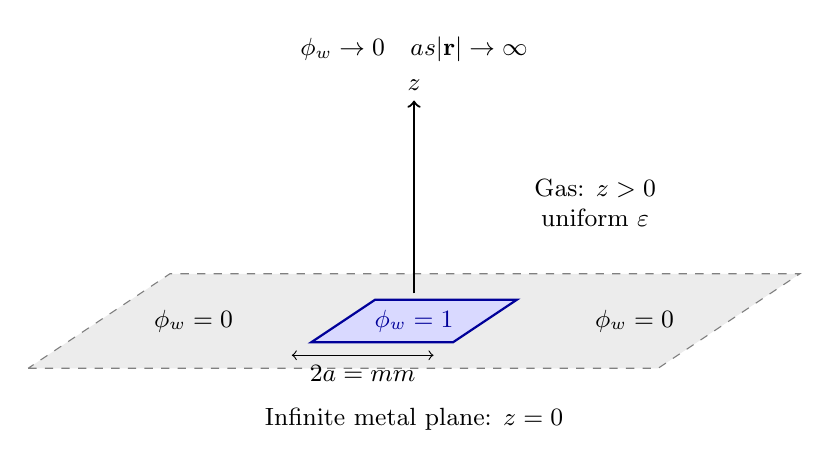
\begin{tikzpicture}[x={(1cm,0cm)},y={(0.45cm,0.3cm)},z={(0cm,1cm)},
                    font=\small]
 \fill[gray!15] (-4,-2,0) -- (4,-2,0) -- (4,2,0) -- (-4,2,0) -- cycle;
 \draw[dashed,gray] (-4,-2,0) -- (4,-2,0) -- (4,2,0) -- (-4,2,0) -- cycle;
 \filldraw[fill=blue!15,draw=blue!60!black,thick]
   (-0.9,-0.9,0) -- (0.9,-0.9,0) -- (0.9,0.9,0) -- (-0.9,0.9,0) -- cycle;
 \node[blue!60!black] at (0,0,0) {$\phi_w=1$};
 \node at (-2.8,0,0) {$\phi_w=0$};
 \node at (2.8,0,0) {$\phi_w=0$};
 \draw[->,thick] (0,0,0.35) -- (0,0,2.8) node[above] {$z$};
 \node[align=center] at (2.3,0,1.5) {Gas: $z>0$\\uniform $\varepsilon$};
 \node at (0,0,3.45)
   {$\phi_w\to0\quad\text{as }|\mathbf r|\to\infty$};
 \draw[<->] (-0.9,-1.45,0) -- (0.9,-1.45,0)
   node[midway,below] {$2a=\SI{\SignalPadWidth}{mm}$};
 \node at (0,0,-1.25) {Infinite metal plane: $z=0$};
\end{tikzpicture}
